%%%%%%%%%%%%%%%%%%%%%%%%%%%%%%%%%%%%%%%%%%%%%%%%
%%%%%%%%%%%%%%%%%%%%%%%%%%%%%%%%%%%%%%%%%%%%%%%%
\documentclass[11pt]{article}

%%%%%%%%%%%%%%%%%%%%%%%%%%%%%%%%%%%%%%%%%%%%%%%%
% Package UPSTI_Document
%%%%%%%%%%%%%%%%%%%%%%%%%%%%%%%%%%%%%%%%%%%%%%%% 
\usepackage{UPSTI_Document}
\usepackage{hyperref}
\usepackage{placeins}
\hypersetup{
    colorlinks=true,
    linkcolor=black,
%    filecolor=blue,      
    urlcolor=blue,
}
\urlstyle{same}
\usepackage{placeins}
\usepackage{soul}
\usepackage{longtable}
\usepackage{fancyvrb}


\newcolumntype{M}[1]{>{\centering\arraybackslash}m{#1}}

\setlength{\parskip}{\medskipamount}

\makeatletter
\let\my@minipagerestore\@minipagerestore
\newcommand{\@minipagerestore}{%
  \setlength{\parskip}{\medskipamount}
  \my@minipagerestore
}

\newcommand{\UPSTIvariante}{7}
\newcommand{\UPSTIidTypeDocument}{1}
\newcommand{\UPSTIidVersionDocument}{1} % 2 pour eleve - 1 pour prof
%\newcommand{\UPSTIidClasse}{0}
%\newcommand{\UPSTIidMatiere}{2}
\newcommand{\UPSTInumeroSequence}{1}
\newcommand{\UPSTItitreEnTete}{Graphes~: parcours}      
\newcommand{\UPSTIduree}{} 
\newcommand{\UPSTInumero}{12}
\newcommand{\UPSTIprogramme}{Graphes}
\newcommand{\UPSTInumeroVersion}{1.0}
\UPSTIcompileVars		% "Compile" les variables

\setcounter{tocdepth}{3}     % Dans la table des matieres
\renewcommand{\UPSTIclasse}{PCSI}

\RequirePackage{svg}
\RequirePackage{stmaryrd}
%\RequirePackage{caption}
%\RequirePackage{subcaption}
\graphicspath{ {./images/} }
\RequirePackage[vlined, french, onelanguage]{algorithm2e} 

%%%%%%%%%%%%%%%%%%%%%%%%%%
%DEBUT DU DOCUMENT
%%%%%%%%%%%%%%%%%%%%%%%%%%

\begin{document}

\UPSTIbuildPage

\tableofcontents

\clearpage 

\section{Parcours en largeur}

\subsection{Description et illustration}

\begin{figure}[htb]
	\hfill
	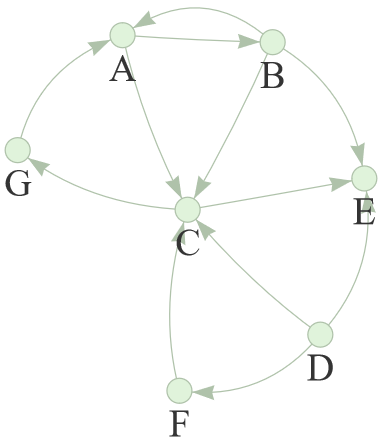
\includegraphics[width=0.19\linewidth]{parcoursLargeurCrop0.png}
	\hfill
	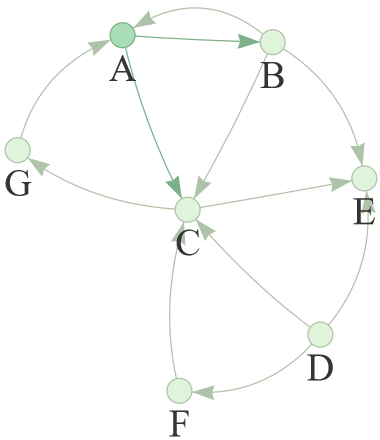
\includegraphics[width=0.19\linewidth]{parcoursLargeurCrop1.png}
	\hfill
	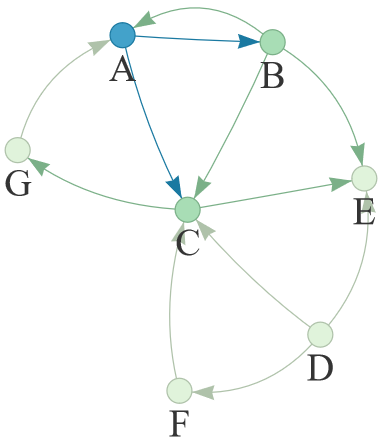
\includegraphics[width=0.19\linewidth]{parcoursLargeurCrop2.png}
	\hfill
	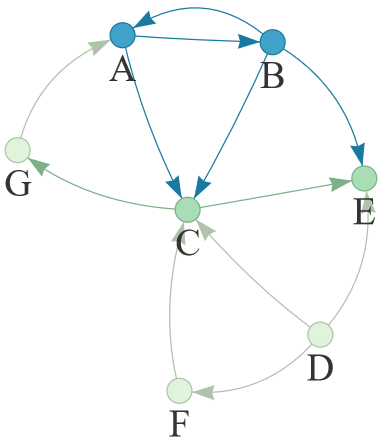
\includegraphics[width=0.19\linewidth]{parcoursLargeurCrop3.png}
	\hfill
	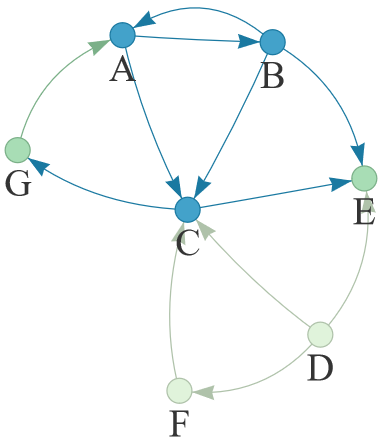
\includegraphics[width=0.19\linewidth]{parcoursLargeurCrop4.png}
	\hfill
	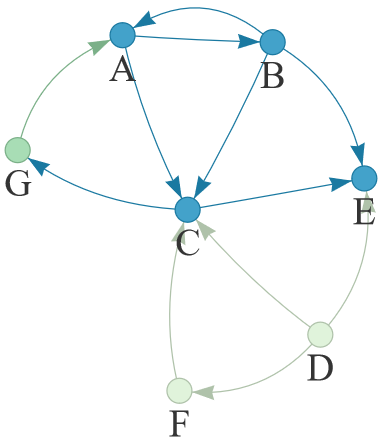
\includegraphics[width=0.19\linewidth]{parcoursLargeurCrop5.png}
	\hfill
	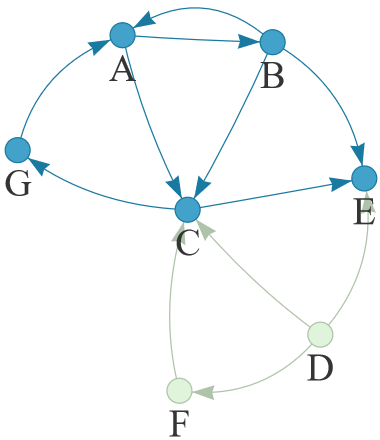
\includegraphics[width=0.19\linewidth]{parcoursLargeurCrop6.png}
	\hfill
	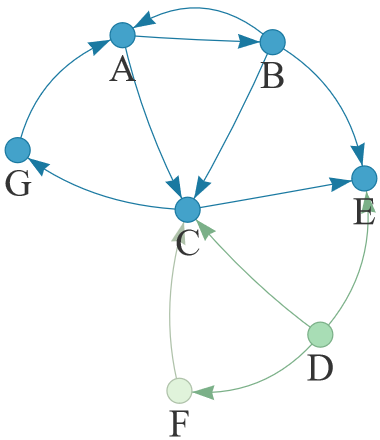
\includegraphics[width=0.19\linewidth]{parcoursLargeurCrop7.png}
	\hfill
	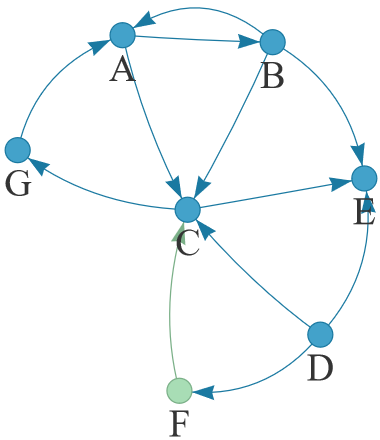
\includegraphics[width=0.19\linewidth]{parcoursLargeurCrop8.png}
	\hfill
	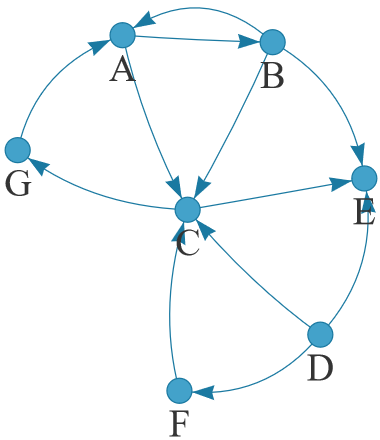
\includegraphics[width=0.19\linewidth]{parcoursLargeurCrop9.png}
	\hfill
	\caption{Illustration du parcours en largeur}
	\label{fig:parcoursLargeur}
\end{figure}

Le parcours en largeur (ou BFS, pour \emph{Breadth First Search}) explore un graphe en considérant tous les successeurs d'un sommet exploré. On utilise une file pour stocker les différents sommets à explorer~: quand on rencontre un nouveau sommet, on l'enfile, et on retire de la file pour savoir par où avancer. On part d'un sommet racine qui sera le premier à être mis en queue. On marque les sommets déjà explorés afin de ne pas effectuer un même parcours plusieurs fois. On a fini l'exploration à partir d'une racine donnée si la file est vide. Si, à partir d'une racine, tout le graphe n'a pas été parcouru, on recommence avec une nouvelle racine non-marquée.

\subsection{État de la file}

Les états successifs de la file sur les différentes étapes sont les suivantes dans l'illustration de la \UPSTIfig{fig:parcoursLargeur}.

\begin{center}
	\begin{tabular}{|c|c|c|c|c|c|c|c|c|c|c|}
		\hline
		Étape & 1 & 2 & 3 & 4 & 5 & 6 & 7 & 8 & 9 & 10 \\
		\hline
		File & [] & [A] & [B,C] & [C,E] & [E,G] & [G] & [] & [D] & [F] & [] \\
		\hline
	\end{tabular}
\end{center}

\newpage

\subsection{Pseudo-code}

Le codage de cet algorithme peut se faire avec 2 sous-parties~: 
\begin{itemize}
	\item un algorithme d'exploration en largeur à partir d'un sommet, 
	\item le parcours en largeur qui appelle l'algorithme d'exploration pour chaque racine pas encore explorée.
\end{itemize}

Le pseudo-code correspondant à l'exploration en largeur est le suivant~:
\begin{algorithm}
	\Entree{Graphe G, Sommet r}
	f reçoit une file vide\;
	r enfilé dans f \;
	r marqué comme parcouru \;
	\Tq{f est non vide}
	{
		s retiré de la file\;
		\PourCh{successeur ss de s dans G}
		{
			\Si{ss marqué comme non-parcouru}{
				ss enfilé dans f \;
				ss marqué comme parcouru \;
			}
		}
	}
\caption{Exploration en largeur à partir d'une racine r}
\end{algorithm}

Le pseudo-code correspondant au parcours complet est le suivant~:
\begin{algorithm}
	\Entree{Graphe G}
	\PourCh{sommet s dans les sommets de G}
	{
		s marqué comme non-parcouru\;
	}
	\PourCh{racine r dans les sommets de G}
	{
		\If{r marqué comme non-parcouru}
		{
			explorationLargeur(G, r) \;
		}
	}
\caption{Parcours en largeur complet}
\end{algorithm}

\FloatBarrier



\subsection{Implémentation en Python}

On considère ici le graphe en entrée comme étant un dictionnaire d'adjacence. Pour consigner le marquage des sommets, on choisit d'utiliser un dictionnaire de booléens.

\lstinputlisting[lastline=20]{programmes/parcoursLargeur2.py}

\section{Parcours en profondeur}

\subsection{Description et illustration}

\begin{figure}[htb]
	\hfill
	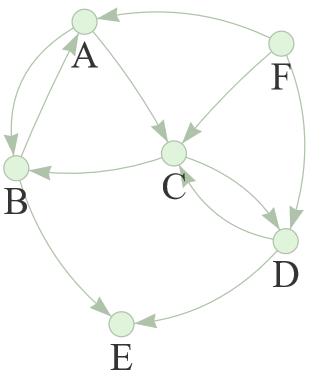
\includegraphics[width=0.16\linewidth]{parcoursProfondeurCrop0.png}
	\hfill
	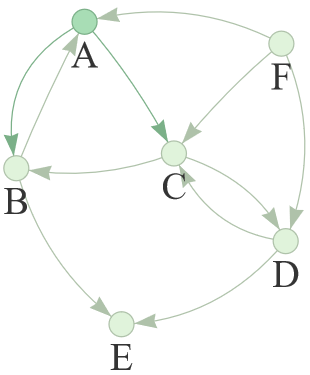
\includegraphics[width=0.16\linewidth]{parcoursProfondeurCrop1.png}
	\hfill
	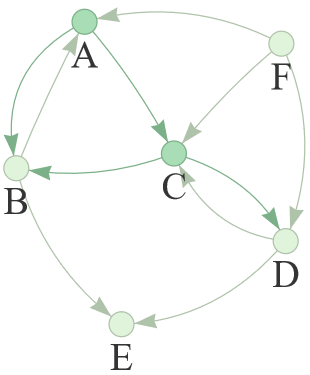
\includegraphics[width=0.16\linewidth]{parcoursProfondeurCrop2.png}
	\hfill
	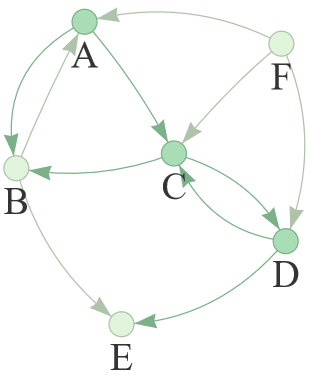
\includegraphics[width=0.16\linewidth]{parcoursProfondeurCrop3.png}
	\hfill
	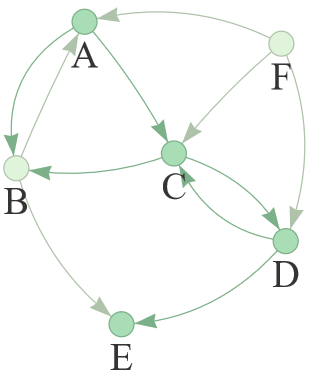
\includegraphics[width=0.16\linewidth]{parcoursProfondeurCrop4.png}
	\hfill
	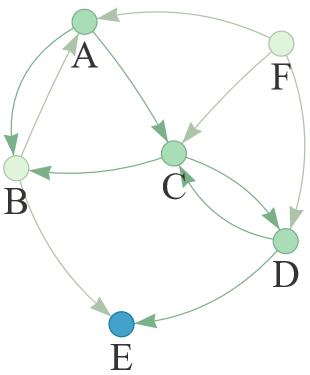
\includegraphics[width=0.16\linewidth]{parcoursProfondeurCrop5.png}
	\hfill
	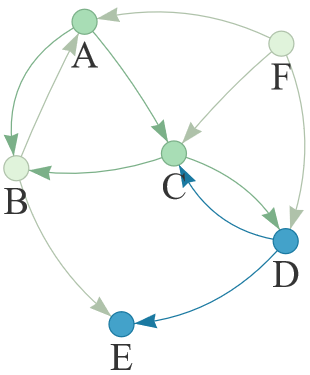
\includegraphics[width=0.16\linewidth]{parcoursProfondeurCrop6.png}
	\hfill
	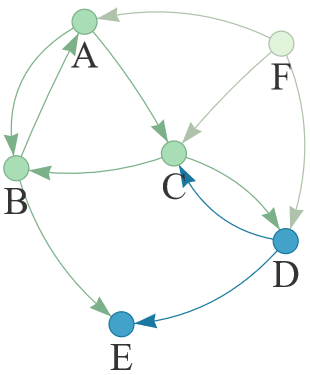
\includegraphics[width=0.16\linewidth]{parcoursProfondeurCrop7.png}
	\hfill
	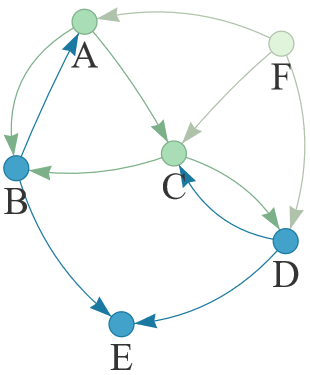
\includegraphics[width=0.16\linewidth]{parcoursProfondeurCrop8.png}
	\hfill
	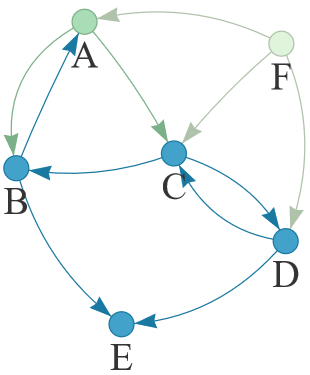
\includegraphics[width=0.16\linewidth]{parcoursProfondeurCrop9.png}
	\hfill
	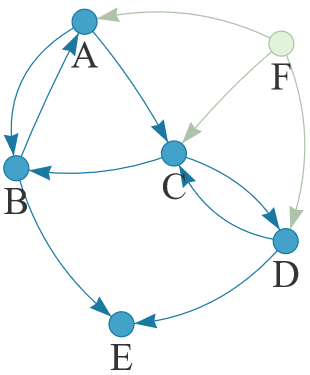
\includegraphics[width=0.16\linewidth]{parcoursProfondeurCrop10.png}
	\hfill
	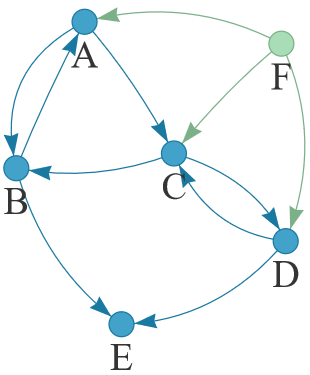
\includegraphics[width=0.16\linewidth]{parcoursProfondeurCrop11.png}
	\hfill
%	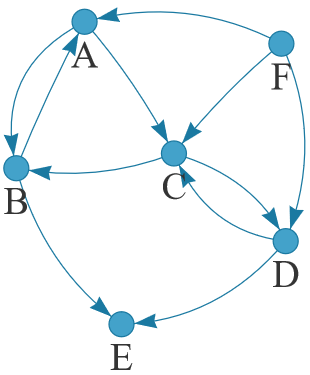
\includegraphics[width=0.16\linewidth]{parcoursProfondeurCrop12.png}
%	\hfill
	\caption{Illustration du parcours en profondeur}
	\label{fig:parcoursProfondeur}
\end{figure}

Le parcours en profondeur (ou DFS, pour \emph{Depth First Search}) explore un graphe en considérant un seul successeur d'un sommet exploré à la fois. On utilise une pile pour stocker les différents sommets à explorer~: quand on rencontre un nouveau sommet, on l'empile. Quand un sommet n'a pas ou plus de voisin non-marqué, on peut le dépiler. On part d'un sommet racine qui sera le premier à être empiler. On marque les sommets déjà explorés afin de ne pas effectuer un même parcours plusieurs fois. On a fini l'exploration à partir d'une racine donnée si la pile est vide. Si, à partir d'une racine, tout le graphe n'a pas été parcouru, on recommence avec une nouvelle racine non-marquée.

\subsection{État de la pile}

Les états successifs de la pile sur les différentes étapes sont les suivantes dans l'illustration de la \UPSTIfig{fig:parcoursProfondeur}.

\begin{center}
	\begin{tabular}{|c|c|c|c|c|c|c|c|c|c|c|c|c|}
		\hline
		Étape & 1 & 2 & 3 & 4 & 5 & 6 & 7 & 8 & 9 & 10 & 11 & 12 \\
		\hline
		Pile & [] & [A] & [A,C] & [A,C,D] & [A,C,D,E] & [A,C,D] & [A,C] & [A,C,B] & [A,C] & [A] & [] & [F] \\
		\hline
	\end{tabular}
\end{center}

\newpage

\subsection{Pseudo-code}

Le codage de cet algorithme peut se faire avec 2 sous-parties~: 
\begin{itemize}
	\item un algorithme d'exploration en profondeur à partir d'une pile de sommets, codé récursivement, 
	\item le parcours en profondeur qui appelle l'algorithme d'exploration pour chaque racine pas encore explorée.
\end{itemize}

Le pseudo-code correspondant est donc le suivant~:

\begin{algorithm}
	\Entree{Graphe G, pile de sommets p}
	s valeur du haut de la pile p \;
	s marqué comme parcouru \;
	\PourCh{successeur ss de s dans G}
	{
		\Si{ss n'est pas marqué}
		{
			ss empilé dans p \;
			explorationProfondeur(G, p)
		}
	}
	s enlevé de la pile p \;
\caption{Exploration en profondeur avec pile}
\end{algorithm}

\begin{algorithm}
	\Entree{Graphe G}
	\PourCh{sommet s dans les sommets de G}
	{
		s marqué comme non-parcouru\;
	}
	\PourCh{racine r dans les sommets de G}
	{
		\If{r marqué comme non-parcouru}
		{
			p reçoit une pile vide \;
			r empilé dans p \;
			explorationPronfondeur(G, p) \;
		}
	}
	\caption{Parcours en profondeur complet}
\end{algorithm}

\FloatBarrier


\subsection{Implémentation en Python}

On considère ici le graphe en entrée comme étant un dictionnaire d'adjacence. Pour consigner le marquage des sommets, on choisit d'utiliser un dictionnaire de booléens.

\lstinputlisting[lastline=17]{programmes/parcoursProfondeur2.py}

La pile de sommets peut être interne et ne pas être explicité~: en effet, cette pile de sommets correspond à la pile d'appels récursifs, et on peut donc ne pas expliciter cette pile.

\lstinputlisting[lastline=13]{programmes/parcoursProfondeur3.py}


\UPSTIattention{
	Les implémentations des algorithmes de parcours présentés ici n'ont rien d'officiel. De nombreuses variantes existent, et nous n'allons pas toutes les présenter. 
}

\UPSTIaRetenir{
	Ce qu'il est fondamental de retenir sur le parcours de graphe~:
	\begin{itemize}
		\item il est primordial de laisser des marques de son passage par un graphe afin de ne pas être enfermé dans des boucles infinies causées par des circuits (dans un graphe orienté) ou des cycles (dans un graphe non-orienté)~; 
		\item le parcours en largeur se base sur l'utilisation d'une file, forcément explicite~; 
		\item le parcours en profondeur se base sur l'utilisation d'une pile, qui doit forcément être explicité dans un codage non-récursif, mais qui peut être implicite dans un codage récursif. 
	\end{itemize}
}


\section{Utilisation des parcours}

Les parcours sont au c\oe{}ur de la résolution de nombreux problèmes dans les graphes~: 
\begin{itemize}
	\item détermination des composantes connexes dans un graphe non orienté~; 
	\item existence et obtention d'un chemin d'un sommet à un autre~; 
	\item obtention du plus court chemin d'un sommet à un autre~;
	\item existence d'un cycle dans un graphe non orienté ou d'un circuit dans un  graphe orienté~;
	\item etc.
\end{itemize}

Dans chaque cas, il faudra enrichir un des deux algorithmes de base pour obtenir les informations souhaitées. Si quelques cas vont être traité en cours, les Travaux Pratiques complèteront cet aperçu. 

\subsection{Détermination des composantes connexes dans un graphe non orienté}

Dans un graphe non orienté, le parcours à partir d'une racine permet d'atteindre la totalités des sommets de la composante connexe qui contient cette racine~: on peut donc, pour cet algorithme, enrichir soit le parcours en largeur, soit le parcours en profondeur. 

On peut ainsi attribuer à chaque sommet un numéro caractérisant la composante connexe, numéro provenant d'un compteur. Ce compteur est incrémenté à chaque fois qu'une nouvelle composante connexe est visitée.

Proposer une implémentation à partir du parcours en largeur~: 

\UPSTIcorrection{
\lstinputlisting[lastline=26]{programmes/NumeroterComposante.py}
}

\newpage

%\subsection{Distance minimale d'un sommet à une racine}
%En enrichissant l'algorithme de parcours en largeur, on peut obtenir la distance minimale en nombre d'arcs d'un sommet $s_0$ à la racine $r$. On va noter~: 
%\begin{itemize}
%	\item $d(s_0)$, la distance minimale du sommet $s_0$ à la racine $r$~;
%	\item $p(s_0)$, le prédecesseur de $s_0$ sur le plus court chemin provenant de $r$.
%\end{itemize}
%
%En pratique, $d(s_0)$ est initialisé à 0 en début de parcours, puis incrémenté de 1 à chaque descente à  un niveau inférieur, c'est-à-dire dès que tous les  successeurs d'un sommet sont intégrés à la file. Le dictionnaire du prédécesseur de chaque sommet est conservé, permettant ainsi de reconstituer le chemin à distance minimale entre $r$ et $s_0$.

\subsection{Existence d'un circuit dans un graphe orienté}

En modifiant légèrement un parcours en profondeur d'un graphe, on peut détecter la présence d'un circuit. En effet, si on se retrouve lors du parcours à rencontrer un sommet déjà dans la pile, alors le graphe comporte un circuit.

Proposer une implémentation~: 

\UPSTIcorrection{
	\lstinputlisting[lastline=18]{programmes/presenceCircuit.py}
}

\newpage

%\subsection{Existence d'un cycle dans un graphe non orienté}
%
%En enrichissant l'algorithme de recherche en profondeur, on peut déterminer la présence d'un cycle dans un graphe non orienté. En effet, on peut avoir 4 types de successeurs à $s$~:
%\begin{itemize}
%	\item successeur marqué et hors de la pile~: à ignorer~;
%	\item marqué et parent de $s$~: à ignorer~;
%	\item non-marqué~: continuation classique de l'algorithme~;
%	\item marqué, dans la pile et non-parent~: cela correspond donc à un cycle.
%\end{itemize}
%
%Le graphe G non orienté et connexe contient un cycle si, à une étape de son parcours, le sommet $s$ de la pile (dernier sommet marqué) a un successeur déjà présent dans la pile, soit un successeur marqué qui n'est pas non plus son prédécesseur. 
%
%Une façon simple pour détecter cela en temps constant sans changer profondément l'algorithme de recherche est de mettre en place un marquage à 3 niveaux. On différencie ainsi~:
%\begin{itemize}
%	\item les sommets entièrement non-visités,
%	\item les sommets en cours de visite (dans la pile), 
%	\item les sommets dont la visite est fini (sortis de la pile).
%\end{itemize}
%
%	On peux coder cela par des chiffres (mais ce n'est pas très explicite) ou par des caractères, par exemple \texttt{'attente'}, \texttt{'découvert'}, \texttt{'exploré'}).

%\begin{lstlisting}
%	for cle in d:
%	    uneClee = cle
%	    break
%\end{lstlisting}


%\UPSTIremarque[Obtention d'un élément quelconque d'un dictionnaire]{
%	Si on souhaite obtenir un élément d'un itérable, comme par exemple une clé d'un dictionnaire, on peut utiliser une conversion en liste par exemple~:
%	
%	\noindent \texttt{uneCle = list(d.keys())[0]} ou, en plus compact,  \texttt{uneCle = list(d)[0]}.
%	
%	\noindent Mais la conversion en liste des clés d'un dictionnaire possède un coût linéaire, ce qui n'est pas a priori nécessaire pour trouver une seule clé dans un dictionnaire~: on préférera donc un parcours sur un seul élément~:
%	
%	\noindent \texttt{for cle in d:} \\
%	\texttt{\phantom{mmmm}uneCle = cle} \\
%	\texttt{\phantom{mmmm}break}
%
%	\noindent On a alors un coût constant, car on arrête la recherche d'une clé au premier élément trouvé. 
%}

\end{document}